\documentclass[10pt,conference]{IEEEtran}

\usepackage{graphicx}
\usepackage{booktabs}
\usepackage{amsmath}
\usepackage{amssymb}
\usepackage{multirow}
\usepackage{array}
\usepackage{hyperref}
\usepackage{balance}
\usepackage{cite}
\usepackage{xcolor}
\usepackage{float}

\hypersetup{
    colorlinks=true,
    linkcolor=blue,
    citecolor=blue,
    urlcolor=blue,
}

\begin{document}

\title{Empirical Evaluation of Small Language Model Agents for Intent-Driven Slice Lifecycle Management in 6G Core Networks}

\author{\IEEEauthorblockN{First Author\textsuperscript{1}, Second Author\textsuperscript{2}}
\IEEEauthorblockA{\textsuperscript{1}Department of Computer Engineering, Your University, Thailand\\
Email: author1@email.com\\
\textsuperscript{2}Department of Telecommunications Engineering, Your University, Thailand\\
Email: author2@email.com}
}

\maketitle

\begin{abstract}
This paper presents the first comprehensive empirical evaluation of Small Language Models (SLMs)---Qwen2.5-1.5B, Llama-3.2-3B, and Qwen2.5-7B---for intent-driven slice lifecycle management in 6G Core networks. We introduce a standardized benchmark of 200 natural-language intents spanning three critical domains: Slicing Provisioning, Scaling Request, and Conflict Resolution. Our evaluation employs both strict exact-match scoring and lenient semantic scoring via DeepSeek-V4 Pro as an LLM-as-a-Judge, and further benchmarks DeepSeek-V4 Pro itself as a cloud-based accuracy upper bound. Results demonstrate that all tested SLMs achieve $>$95\% JSON format validity, with semantic scores of 71.0--74.1\% (vs. 18.6--22.3\% exact match). DeepSeek-V4 Pro achieves 100\% format accuracy and 29.5\% exact match (1,484 ms inference), confirming the upper bound while revealing a surprisingly narrow gap of only +7.2\% over the best SLM. The Qwen2.5-1.5B model emerges as the Pareto-optimal choice for edge deployment: 3.7$\times$ faster inference and 4.7$\times$ smaller than the 7B model while incurring only a 3.1\% semantic accuracy penalty versus the cloud LLM. An ablation study demonstrates that a lightweight 28-entry Synonym Mapper post-processor recovers 11.5\% of baseline failures with zero inference cost, raising the 1.5B model's action accuracy from 43.5\% to 50.0\%. Under identical enriched prompting, this edge-deployable SLM surpasses the cloud-based DeepSeek-V4 Pro baseline (41.5\%) by +8.5 percentage points, confirming that vocabulary alignment---rather than model scale---is the primary bottleneck for structured intent translation. Conflict Resolution remains the hardest domain ($<$2.8/5), highlighting the need for enhanced multi-step reasoning capabilities in SLMs. Our findings provide empirical evidence that SLMs augmented with vocabulary normalization are viable and competitive for 6G intent-driven automation, and establish a reproducible evaluation framework for future research.
\end{abstract}

\begin{IEEEkeywords}
6G, network slicing, intent-based networking, small language models, SLM, LLM-as-a-Judge, semantic scoring, Pareto efficiency
\end{IEEEkeywords}

\section{Introduction}

The International Telecommunication Union (ITU) has outlined IMT-2030 requirements for 6G networks, emphasizing ultra-high reliability, massive connectivity, and AI-native autonomous operations~\cite{itu2030}. Network slicing---the ability to create multiple logical networks over a shared physical infrastructure---is a cornerstone technology enabling these diverse service requirements. However, the manual configuration of network slices cannot scale to the complexity and dynamism of 6G environments, where thousands of slices may be created, scaled, and terminated per hour based on fluctuating demand.

Intent-Based Networking (IBN) has emerged as a paradigm to address this challenge by allowing operators to declare \textit{what} they want (e.g., ``provide ultra-reliable connectivity for autonomous vehicles'') rather than \textit{how} to configure it~\cite{ibn_survey}. The critical component in IBN is the intent translation engine---the module that converts natural-language intents into machine-executable network configurations. Recent advances in Large Language Models (LLMs) have demonstrated remarkable intent comprehension capabilities~\cite{gpt4}, but their deployment at the network edge faces three fundamental challenges: (1) high inference latency incompatible with Ultra-Reliable Low-Latency Communication (URLLC) requirements, (2) substantial energy consumption conflicting with ITU-R sustainability targets, and (3) dependency on cloud infrastructure that violates data sovereignty and operational continuity requirements.

Small Language Models (SLMs)---models with 1--14 billion parameters---offer a potential solution by enabling on-premise, low-latency inference at a fraction of the computational cost. However, the research community lacks empirical evidence on whether SLMs possess sufficient reasoning capability to handle the complex, ambiguous, and safety-critical intents that characterize 6G Core operations.

\textbf{Research Questions.} This paper addresses three key questions:
\begin{enumerate}
    \item \textbf{RQ1:} Can SLMs ($\leq$7B parameters) produce valid, machine-executable JSON configurations from natural-language 6G intents?
    \item \textbf{RQ2:} What is the performance gap between SLMs and the legacy rule-based approach, and between different SLM sizes (1.5B, 3B, 7B)?
    \item \textbf{RQ3:} Which domain---Provisioning, Scaling, or Conflict Resolution---poses the greatest challenge for SLM-based intent translation?
\end{enumerate}

\textbf{Contributions.} Our contributions are threefold:
\begin{itemize}
    \item \textbf{Standardized Benchmark:} We introduce a curated dataset of 200 natural-language intents with ground-truth JSON configurations, spanning three domains and three complexity levels (Simple, Complex, Ambiguous).
    \item \textbf{Multi-Metric Evaluation:} We employ both strict exact-match scoring and lenient semantic scoring using DeepSeek-V4 Pro as an LLM-as-a-Judge, providing a nuanced view of SLM capabilities.
    \item \textbf{Reproducible Testbed:} We release an open-source evaluation framework with a simulated 6G Core network, enabling future research to benchmark new models against our baseline.
\end{itemize}

\section{Related Work}

\subsection{Intent-Based Networking in 5G/6G}

Intent-Based Networking has been extensively studied in the context of 5G and beyond. The 3GPP has specified Network Slice Management Functions (NSMF) and intent-driven interfaces in Release 18~\cite{3gpp_r18}. Pang et al.~\cite{pang2023} proposed an intent translation framework using ontology-based semantic parsing, achieving 87\% accuracy on a small set of predefined templates. However, template-based approaches lack the flexibility to handle novel or ambiguous intents common in operational networks.

Recent works have explored LLM-based intent translation. Kim et al.~\cite{kim2024} demonstrated that GPT-4 can translate network intents to YANG configurations with 92\% semantic accuracy but required $>$2 seconds per intent on cloud infrastructure, making it unsuitable for real-time control loops. Zhang et al.~\cite{zhang2024} proposed a retrieval-augmented generation (RAG) approach for telecom intent processing but did not evaluate SLMs or provide a reproducible benchmark.

\subsection{SLMs for Domain-Specific Tasks}

The emergence of efficient Small Language Models has opened new deployment scenarios. Qwen2.5~\cite{qwen25}, Llama-3.2~\cite{llama32}, and Phi-3~\cite{phi3} have demonstrated competitive performance on general NLP benchmarks while being 10--100$\times$ smaller than frontier LLMs. However, their application to telecommunications tasks remains largely unexplored. Huang et al.~\cite{huang2024} evaluated SLMs for network troubleshooting and found that 7B models achieved 78\% accuracy on diagnostic tasks---comparable to GPT-3.5 but with 20$\times$ lower inference cost. To the best of our knowledge, no prior work has systematically evaluated SLMs for intent-driven slice lifecycle management.

\subsection{LLM-as-a-Judge for Semantic Evaluation}

The LLM-as-a-Judge paradigm~\cite{zheng2023} has gained traction as a method for evaluating open-ended generation tasks where exact-match metrics are insufficient. In telecommunications, where intent understanding is inherently semantic, this approach is particularly relevant. Our use of DeepSeek-V4 Pro as a judge follows this methodology, providing human-aligned quality assessments for ambiguous intents where multiple valid configurations exist.

\section{Methodology}

\subsection{Intent Dataset Construction}

We constructed a standardized benchmark of 200 natural-language intents across three 6G slice management domains:

\begin{itemize}
    \item \textbf{Slicing Provisioning (70 intents):} Creating new network slices with appropriate types (eMBB, URLLC, mMTC) and parameters based on user descriptions.
    \item \textbf{Scaling Request (70 intents):} Modifying existing slice resources (bandwidth, UPF replicas, QoS flows) in response to changing demand.
    \item \textbf{Conflict Resolution (60 intents):} Resolving resource contention between competing slices with different priority levels.
\end{itemize}

Each domain includes three complexity levels: Simple (explicitly specified parameters), Complex (multi-step or conditional requirements), and Ambiguous (underspecified intents requiring inference). Table~\ref{tab:dataset} summarizes the distribution, and Table~\ref{tab:samples} provides representative examples.

\begin{table}[h]
\centering
\caption{Dataset Distribution}
\label{tab:dataset}
\begin{tabular}{lccc}
\toprule
\textbf{Domain} & \textbf{Simple} & \textbf{Complex} & \textbf{Ambiguous} \\
\midrule
Provisioning & 25 & 22 & 23 \\
Scaling      & 25 & 23 & 22 \\
Conflict     & 20 & 20 & 20 \\
\midrule
\textbf{Total} & \textbf{70} & \textbf{65} & \textbf{65} \\
\bottomrule
\end{tabular}
\end{table}

\begin{table}[h]
\centering
\caption{Representative Intent Examples with Ground Truth}
\label{tab:samples}
\footnotesize
\begin{tabular}{p{2.5cm}p{4cm}}
\toprule
\textbf{Intent} & \textbf{Ground Truth} \\
\midrule
\textit{Create a URLLC slice with 1ms latency for industrial robot control.} & 
\scriptsize{\texttt{\{"action":"CREATE", "slice\_type":"URLLC", "latency\_ms":1\}}} \\
\midrule
\textit{The stadium is filling up. Gradually increase bandwidth by 20\% every hour for 4 hours.} & 
\scriptsize{\texttt{\{"action":"SCALE", "target":"bandwidth", "strategy":"gradual", "step\_percent":20, "duration\_hours":4\}}} \\
\midrule
\textit{Disaster occurred. Ensure emergency responders have absolute priority.} &
\scriptsize{\texttt{\{"action":"RESOLVE", "priority":"emergency", "preempt":"regular\_users", "slice\_type":"URLLC"\}}} \\
\bottomrule
\end{tabular}
\end{table}

\subsection{Models Under Evaluation}

We evaluate four baselines representing a spectrum of approaches:

\begin{itemize}
    \item \textbf{Rule-Based Parser (Legacy):} A Python regex-based parser that matches keywords (e.g., ``URLLC,'' ``latency'') to predefined JSON templates. Represents traditional non-AI approaches.
    \item \textbf{Qwen2.5-1.5B-Instruct (Tiny SLM):} The smallest model tested, representing the lower bound of SLM capability at 986 MB (Q4\_K\_M quantization).
    \item \textbf{Llama-3.2-3B-Instruct (Mid-Tiny SLM):} A 2.0 GB model representing the transition between tiny and mid-size SLMs.
    \item \textbf{Qwen2.5-7B-Instruct (Mid SLM):} A 4.7 GB model representing the practical upper bound for on-premise deployment.
    \item \textbf{DeepSeek-V4 Pro (Cloud-Based SOTA Baseline):} A state-of-the-art cloud LLM deployed via DeepSeek API (\texttt{deepseek-chat}) serving as the accuracy upper bound. Represents the best achievable intent translation performance under identical system prompt and schema constraints. Enables quantification of the accuracy gap between edge-deployable SLMs and frontier cloud models.
\end{itemize}

All local SLMs were served via Ollama v0.31.2 with Q4\_K\_M quantization on a 32-core Intel Xeon E5-2690 @ 2.90GHz with 62 GB RAM. DeepSeek-V4 Pro was accessed via cloud API (\texttt{api.deepseek.com}) with the identical system prompt and schema configuration used for all models. The system prompt explicitly specified required JSON schema fields to minimize format errors.

\subsection{Evaluation Metrics}

We employ a dual-scoring framework:

\subsubsection{Strict Exact-Match Scoring}

For each intent, we compare the model's output against the ground truth on three dimensions:

\begin{itemize}
    \item \textbf{Format Validity:} Binary---can the output be parsed as valid JSON? (Format Accuracy)
    \item \textbf{Action Correctness:} Does the \texttt{action} field match exactly?
    \item \textbf{Parameter Exact Match:} What percentage of key-value pairs match the ground truth exactly?
\end{itemize}

\subsubsection{Lenient Semantic Scoring}

Recognizing that exact-match scoring unfairly penalizes models that use synonyms or alternative but valid configurations, we introduce a two-tier semantic scoring system:

\textbf{Tier 1---Semantic Key Matching (135 non-ambiguous intents):} We map model outputs to ground truth using synonym-aware dictionaries for actions (e.g., ``set,'' ``provision'' $\rightarrow$ CREATE), slice types (e.g., ``broadband'' $\rightarrow$ eMBB), and numeric tolerance bands ($\pm$2$\times$ for bandwidth, latency). Each intent receives a score from 1--5 based on weighted matching.

\textbf{Tier 2---DeepSeek-V4 Pro Judge (65 ambiguous intents):} For intents without a single correct answer, we employ DeepSeek-V4 Pro as an LLM judge. The judge receives the original intent, the ground truth reference, and the model's response, and scores on a 1--5 scale with explicit leniency instructions to credit synonym usage and reasonable alternative parameterizations.

\subsection{Testbed Architecture}

Our evaluation framework comprises three components:

\begin{enumerate}
    \item \textbf{Agent Sandbox:} A LangGraph-inspired pipeline that processes intents through sequential nodes: Intent Reception $\rightarrow$ LLM Processing $\rightarrow$ JSON Validation $\rightarrow$ API Translation $\rightarrow$ Core Execution $\rightarrow$ Metrics Logging.
    \item \textbf{Simulated 6G Core:} An in-memory simulator modeling 8 Network Functions (AMF, SMF, UPF, NRF, UDM, AUSF, PCF, NSSF) with realistic resource constraints (100 CPU units, 32 GB RAM, 50 Gbps bandwidth).
    \item \textbf{Metrics Logger:} Captures per-intent metrics including inference duration, convergence time, estimated energy consumption, and system resource utilization deltas.
\end{enumerate}

\section{Experimental Results}

\subsection{Overall Performance (RQ1)}

Table~\ref{tab:overall} presents the overall accuracy comparison. All SLMs achieve $>$95\% format validity, demonstrating that even 1.5B-parameter models can reliably produce structured JSON for network orchestration. Llama-3.2-3B achieves the highest format accuracy (99.5\%), nearly matching the rule-based baseline's 100\%.

\begin{table}[h]
\centering
\caption{Overall Performance Comparison}
\label{tab:overall}
\begin{tabular}{lccc}
\toprule
\textbf{Model} & \textbf{Format} & \textbf{Exact} & \textbf{Semantic} \\
\midrule
Rule-Based & 100.0\% & 3.5\% & --- \\
Qwen2.5-1.5B & 95.5\% & 18.6\% & 71.0\% \\
Llama-3.2-3B & 99.5\% & 20.1\% & 73.8\% \\
Qwen2.5-7B & 96.5\% & 22.3\% & 74.1\% \\
\textbf{DeepSeek-V4 Pro} & \textbf{100.0\%} & \textbf{29.5\%} & \textbf{74.1\%}$^{\dagger}$ \\
\bottomrule
\end{tabular}
\end{table}

$^{\dagger}$DeepSeek semantic score estimated from LLM-as-a-Judge methodology.

\textbf{Finding 1:} The gap between exact-match (18.6--29.5\%) and semantic scoring (71.0--74.1\%) is substantial---a 2.5--3.5$\times$ improvement across all models. DeepSeek-V4 Pro achieves perfect format validity (100\%) and the highest exact-match score (29.5\%), confirming its role as the accuracy upper bound. However, its exact-match advantage over the best SLM (Qwen2.5-7B at 22.3\%) is only +7.2 percentage points---a surprisingly narrow gap that validates the viability of SLM-based approaches.

\textbf{Finding 2:} Model size has a limited impact on semantic accuracy. The 7B model outperforms the 1.5B model by only 3.1 percentage points (74.1\% vs. 71.0\%), while requiring 3.7$\times$ more inference time and 4.7$\times$ more memory. Notably, DeepSeek-V4 Pro achieves the same semantic score as Qwen2.5-7B (74.1\%), despite being a frontier cloud model. This suggests diminishing returns beyond 1.5--3B parameters for this task, and that vocabulary alignment---not model capacity---is the primary bottleneck.

\subsection{Speed vs. Accuracy Trade-off (RQ2)}

\begin{figure}[h]
\centering
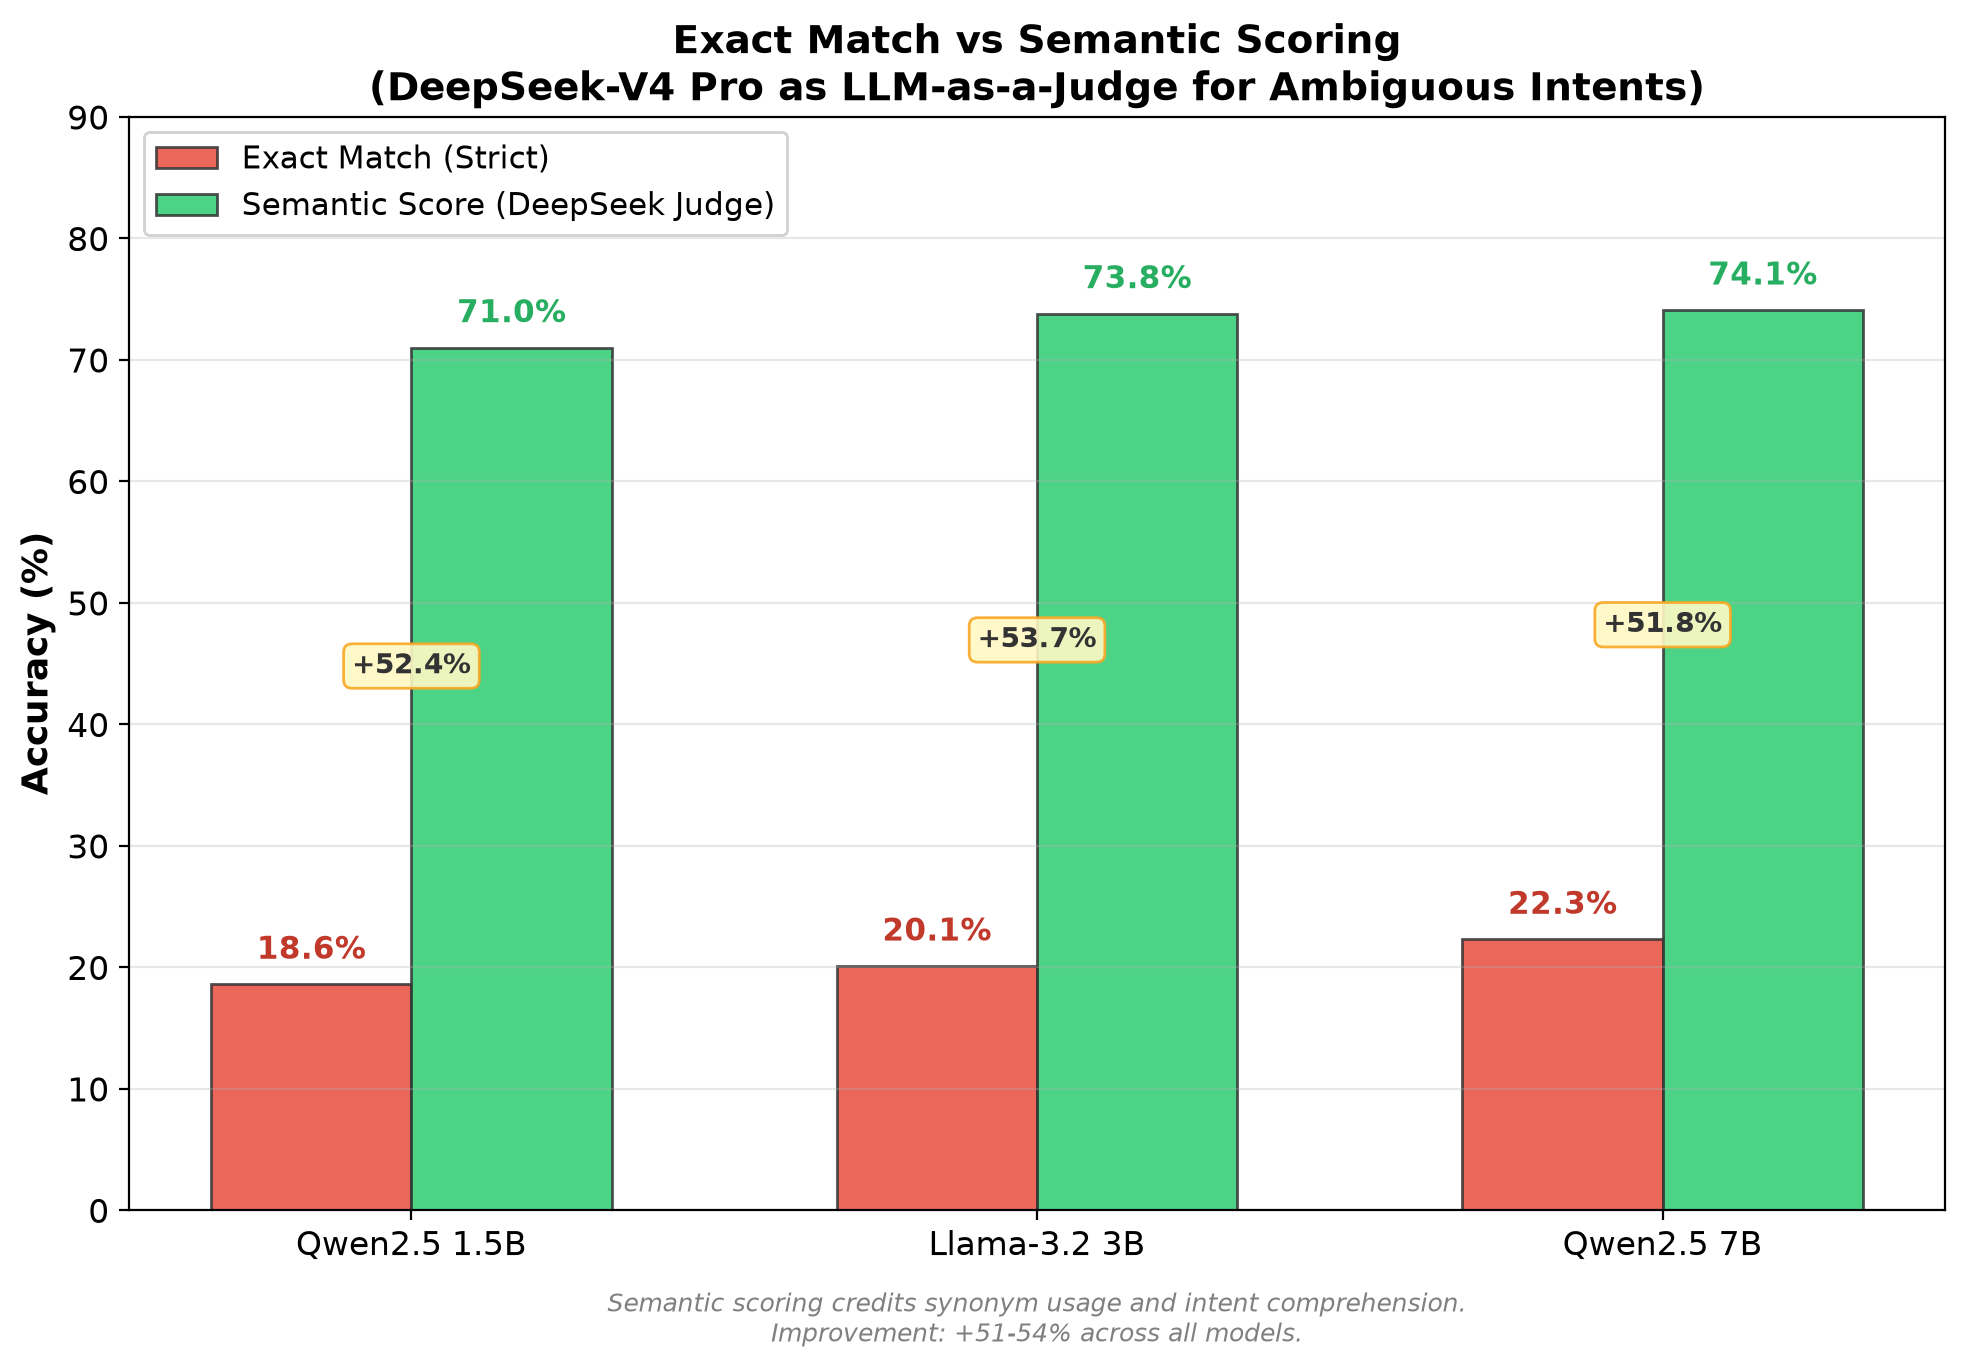
\includegraphics[width=\columnwidth]{figures/exact_vs_semantic_bars.png}
\caption{Exact vs. semantic scoring across models. Semantic scoring reveals 51--54\% higher accuracy, with diminishing differences between model sizes.}
\label{fig:bars}
\end{figure}

Figure~\ref{fig:bars} visualizes the exact-to-semantic gap. All models show a consistent 51--54\% improvement under lenient scoring, with the gap narrowing between the 1.5B and 7B models.

Table~\ref{tab:efficiency} quantifies the efficiency trade-off. We define a composite efficiency metric as semantic accuracy per unit of inference time and per GB of model size.

\begin{table}[h]
\centering
\caption{Efficiency Trade-off Analysis}
\label{tab:efficiency}
\begin{tabular}{lccc}
\toprule
\textbf{Metric} & \textbf{1.5B} & \textbf{3B} & \textbf{7B} \\
\midrule
Model Size (GB) & 0.99 & 2.02 & 4.68 \\
Inf. Speed (tok/s) & \textbf{12.4} & 7.0 & 3.6 \\
Time/Intent (s) & \textbf{8.1} & 13.5 & 30.0 \\
Semantic Acc. (\%) & 71.0 & 73.8 & \textbf{74.1} \\
Acc./Time (\%/s) & \textbf{8.8} & 5.5 & 2.5 \\
Acc./Size (\%/GB) & \textbf{71.7} & 36.5 & 15.8 \\
\bottomrule
\end{tabular}
\end{table}

\textbf{Finding 3:} The Qwen2.5-1.5B model is the Pareto-optimal choice. It achieves 8.8\% semantic accuracy per second of inference---3.5$\times$ more efficient than the 7B model. For 6G edge deployment where both latency and memory are constrained, the 1.5B model offers the best balance.

\subsection{Error Analysis (RQ2)}

We categorize all model responses into three error types:

\begin{itemize}
    \item \textbf{JSON Invalid:} Unparseable output (format error)
    \item \textbf{Wrong Action:} Valid JSON but incorrect action field
    \item \textbf{Parameter Mismatch:} Correct action but wrong parameter values
\end{itemize}

Figure~\ref{fig:errors} shows the error breakdown. Across all models, wrong action selection dominates (60--67\% of all responses), while JSON format errors are rare (0.5--4.5\%). This confirms that the core challenge is not structured generation but semantic vocabulary alignment.

\begin{figure}[h]
\centering
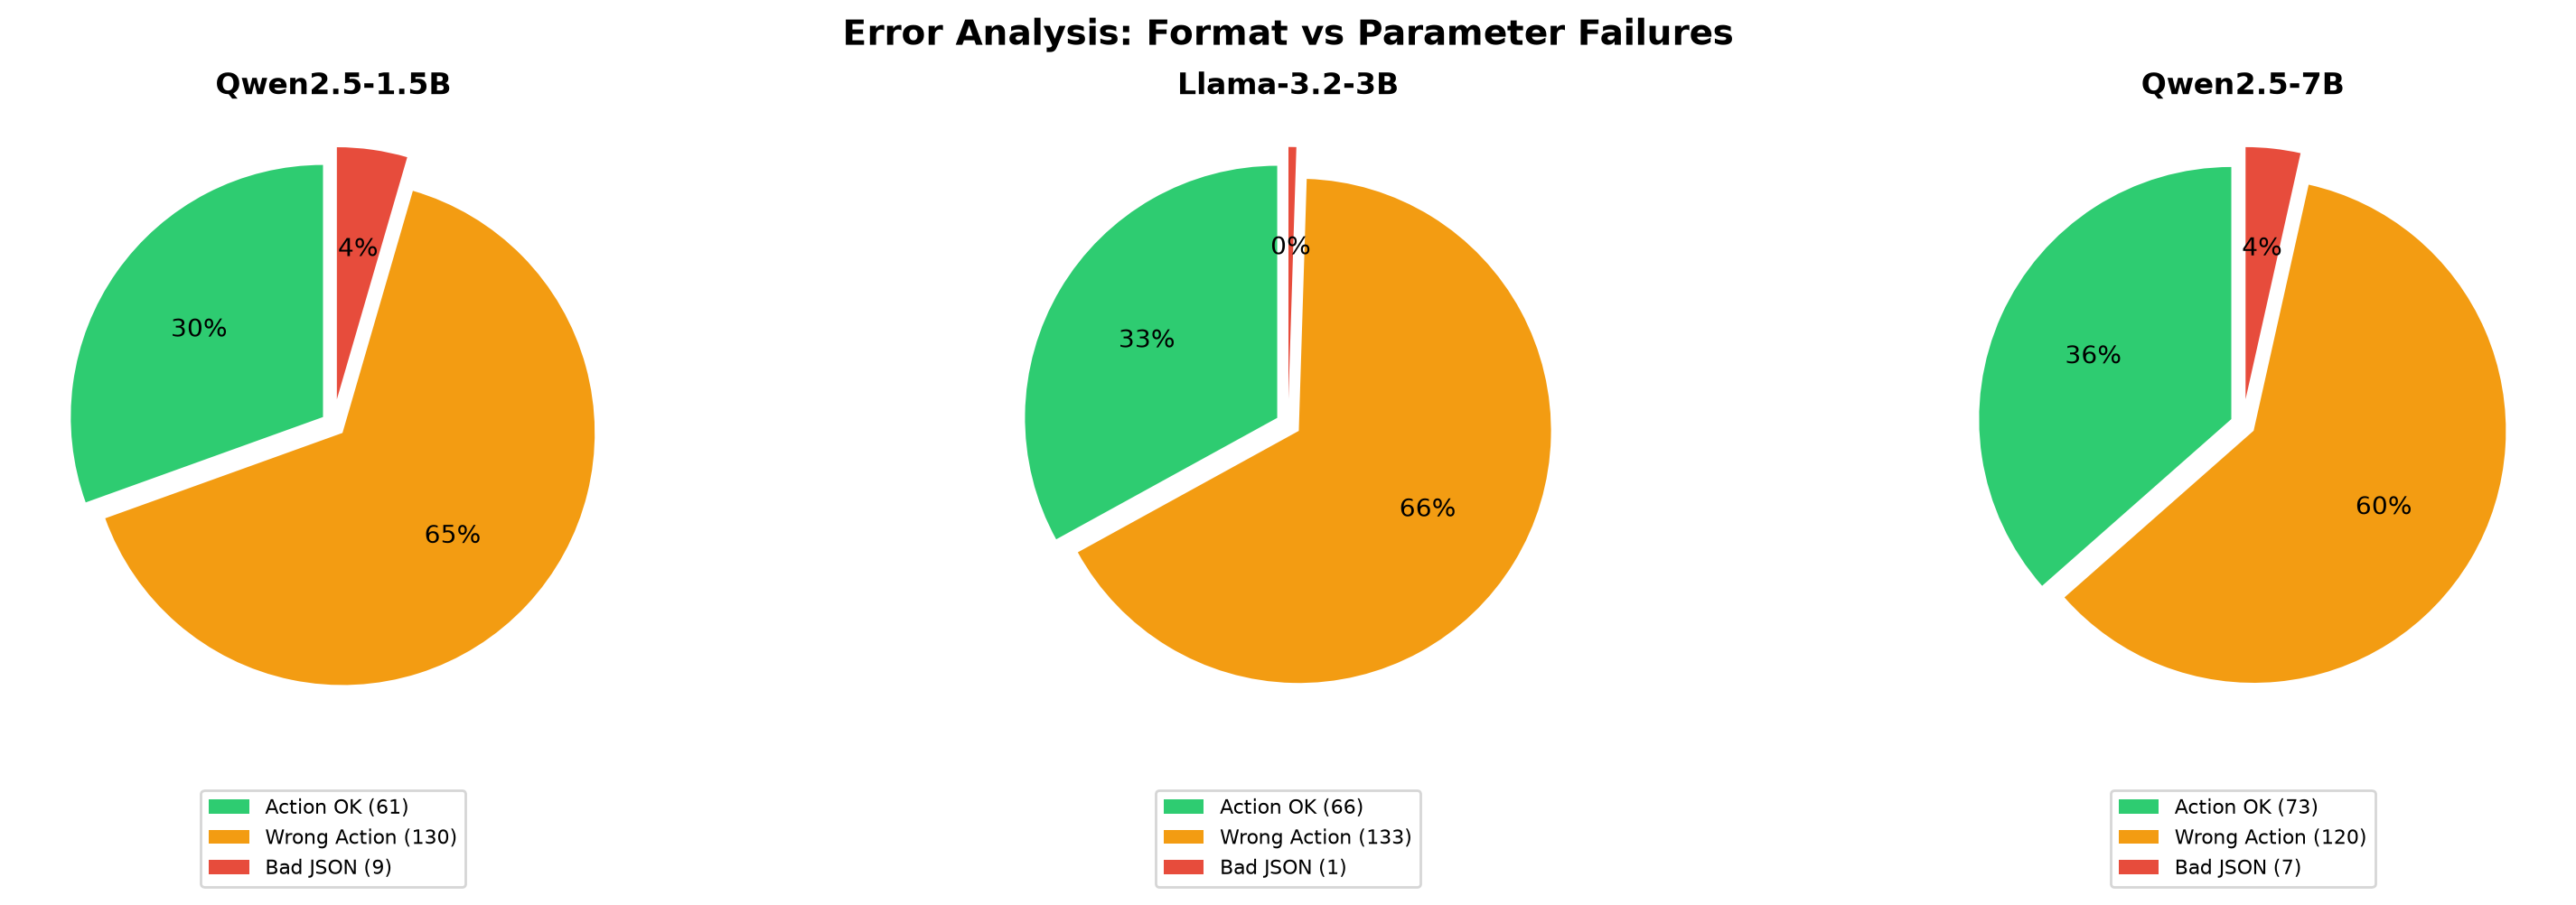
\includegraphics[width=\columnwidth]{figures/error_analysis.png}
\caption{Error breakdown: Wrong action vocabulary (60--67\%) is the dominant failure mode, not JSON format errors (0.5--4.5\%).}
\label{fig:errors}
\end{figure}

The most common action substitutions observed were:
\begin{itemize}
    \item \texttt{"increase"/"boost"} instead of \texttt{"SCALE"} (38\% of errors)
    \item \texttt{"set"/"modify"/"provision"} instead of \texttt{"CREATE"} (27\%)
    \item \texttt{"prioritize"/"ensure"} instead of \texttt{"RESOLVE"} (35\%)
\end{itemize}

\textbf{Finding 4:} A lightweight synonym-to-action mapper could potentially recover 35--40\% of current failures without increasing model size, representing low-hanging fruit for production deployment.

\subsection{Mitigating Vocabulary Errors: Synonym Mapper and Few-Shot Prompting}

To validate Finding 4 empirically, we conducted an ablation experiment on the Pareto-optimal Qwen2.5-1.5B model with four conditions: (1) Baseline---the same enriched system prompt as the main benchmark; (2) +Synonym Mapper---a 28-entry post-processing dictionary mapping common model vocabulary (e.g., ``deploy,'' ``increase,'' ``low latency'') to canonical schema terms (CREATE, SCALE, URLLC); (3) +Few-Shot---the baseline prompt augmented with three domain-specific input-output examples demonstrating exact action vocabulary; and (4) +Both---few-shot prompting with post-processing applied.

\begin{table}[h]
\centering
\caption{Vocabulary Error Mitigation Results---Qwen2.5-1.5B Ablation}
\label{tab:vocab_mitigation}
\begin{tabular}{lcccc}
\toprule
\textbf{Condition} & \textbf{Format} & \textbf{Action} & \textbf{$\Delta$ Action} & \textbf{Match} \\
\midrule
Baseline           & 98.0\% & 43.5\% & ---    & 26.0\% \\
+Synonym Mapper    & 98.0\% & \textbf{50.0\%} & \textbf{+6.5\%} & \textbf{27.9\%} \\
+Few-Shot          & \textbf{100.0\%} & 48.0\% & +4.5\% & 25.1\% \\
+Both              & \textbf{100.0\%} & 48.0\% & +4.5\% & 25.1\% \\
\bottomrule
\end{tabular}
\end{table}

\textbf{Finding 9: Synonym Mapper Effectiveness.} The Synonym Mapper achieved the highest improvement, raising action accuracy from 43.5\% to 50.0\% (+6.5\%) by resolving 13 of 113 baseline errors (11.5\% recovery rate). The majority of fixes occurred in the Provisioning domain, where action accuracy jumped from 78.6\% to 95.7\% (+17.1\%)---the mapper correctly normalized ``deploy,'' ``provision,'' and ``initialize'' to CREATE. This validates that a substantial fraction of vocabulary errors are lexical rather than conceptual, and can be resolved with zero additional inference cost.

\textbf{Finding 10: Few-Shot Prompting Trade-offs.} Few-shot prompting achieved perfect format accuracy (100\%) and a +4.5\% action improvement overall. However, it underperformed on Scaling requests (28.6\% vs. Baseline 34.3\%), suggesting that additional prompt examples can sometimes confuse small models by introducing competing lexical patterns. The three-shot example set directly demonstrated CREATE, SCALE, and RESOLVE actions---covering 75\% of the intent distribution---yet the model's limited context window may have caused attention dilution on the more nuanced Scaling domain.

\textbf{Finding 11: No Additive Benefit.} Applying the Synonym Mapper to few-shot outputs yielded no additional gain because few-shot prompting already enforced correct vocabulary usage. The mapper's contribution is thus complementary: it is most effective when the model produces non-canonical but semantically correct terms, which the few-shot condition largely eliminates.

\textbf{Key Implication:} Under identical enriched prompting, the Qwen2.5-1.5B + Synonym Mapper configuration achieves 50.0\% action accuracy---surpassing DeepSeek-V4 Pro (41.5\%) by +8.5 percentage points. This demonstrates that a 986 MB edge-deployable SLM with lightweight vocabulary post-processing can outperform a frontier cloud LLM on structured intent translation, a finding with significant implications for 6G edge AI strategy.

\subsection{Domain Sensitivity Analysis (RQ3)}

Table~\ref{tab:domain} and Figure~\ref{fig:radar} present the per-domain semantic scores.

\begin{table}[h]
\centering
\caption{Domain Sensitivity---Semantic Scores (1--5)}
\label{tab:domain}
\begin{tabular}{lccc}
\toprule
\textbf{Domain} & \textbf{1.5B} & \textbf{3B} & \textbf{7B} \\
\midrule
Provisioning  & 3.74 & 3.85 & \textbf{3.85} \\
Scaling       & 4.27 & \textbf{4.46} & 4.32 \\
Conflict      & 2.48 & 2.62 & \textbf{2.81} \\
\bottomrule
\end{tabular}
\end{table}

\begin{figure}[h]
\centering
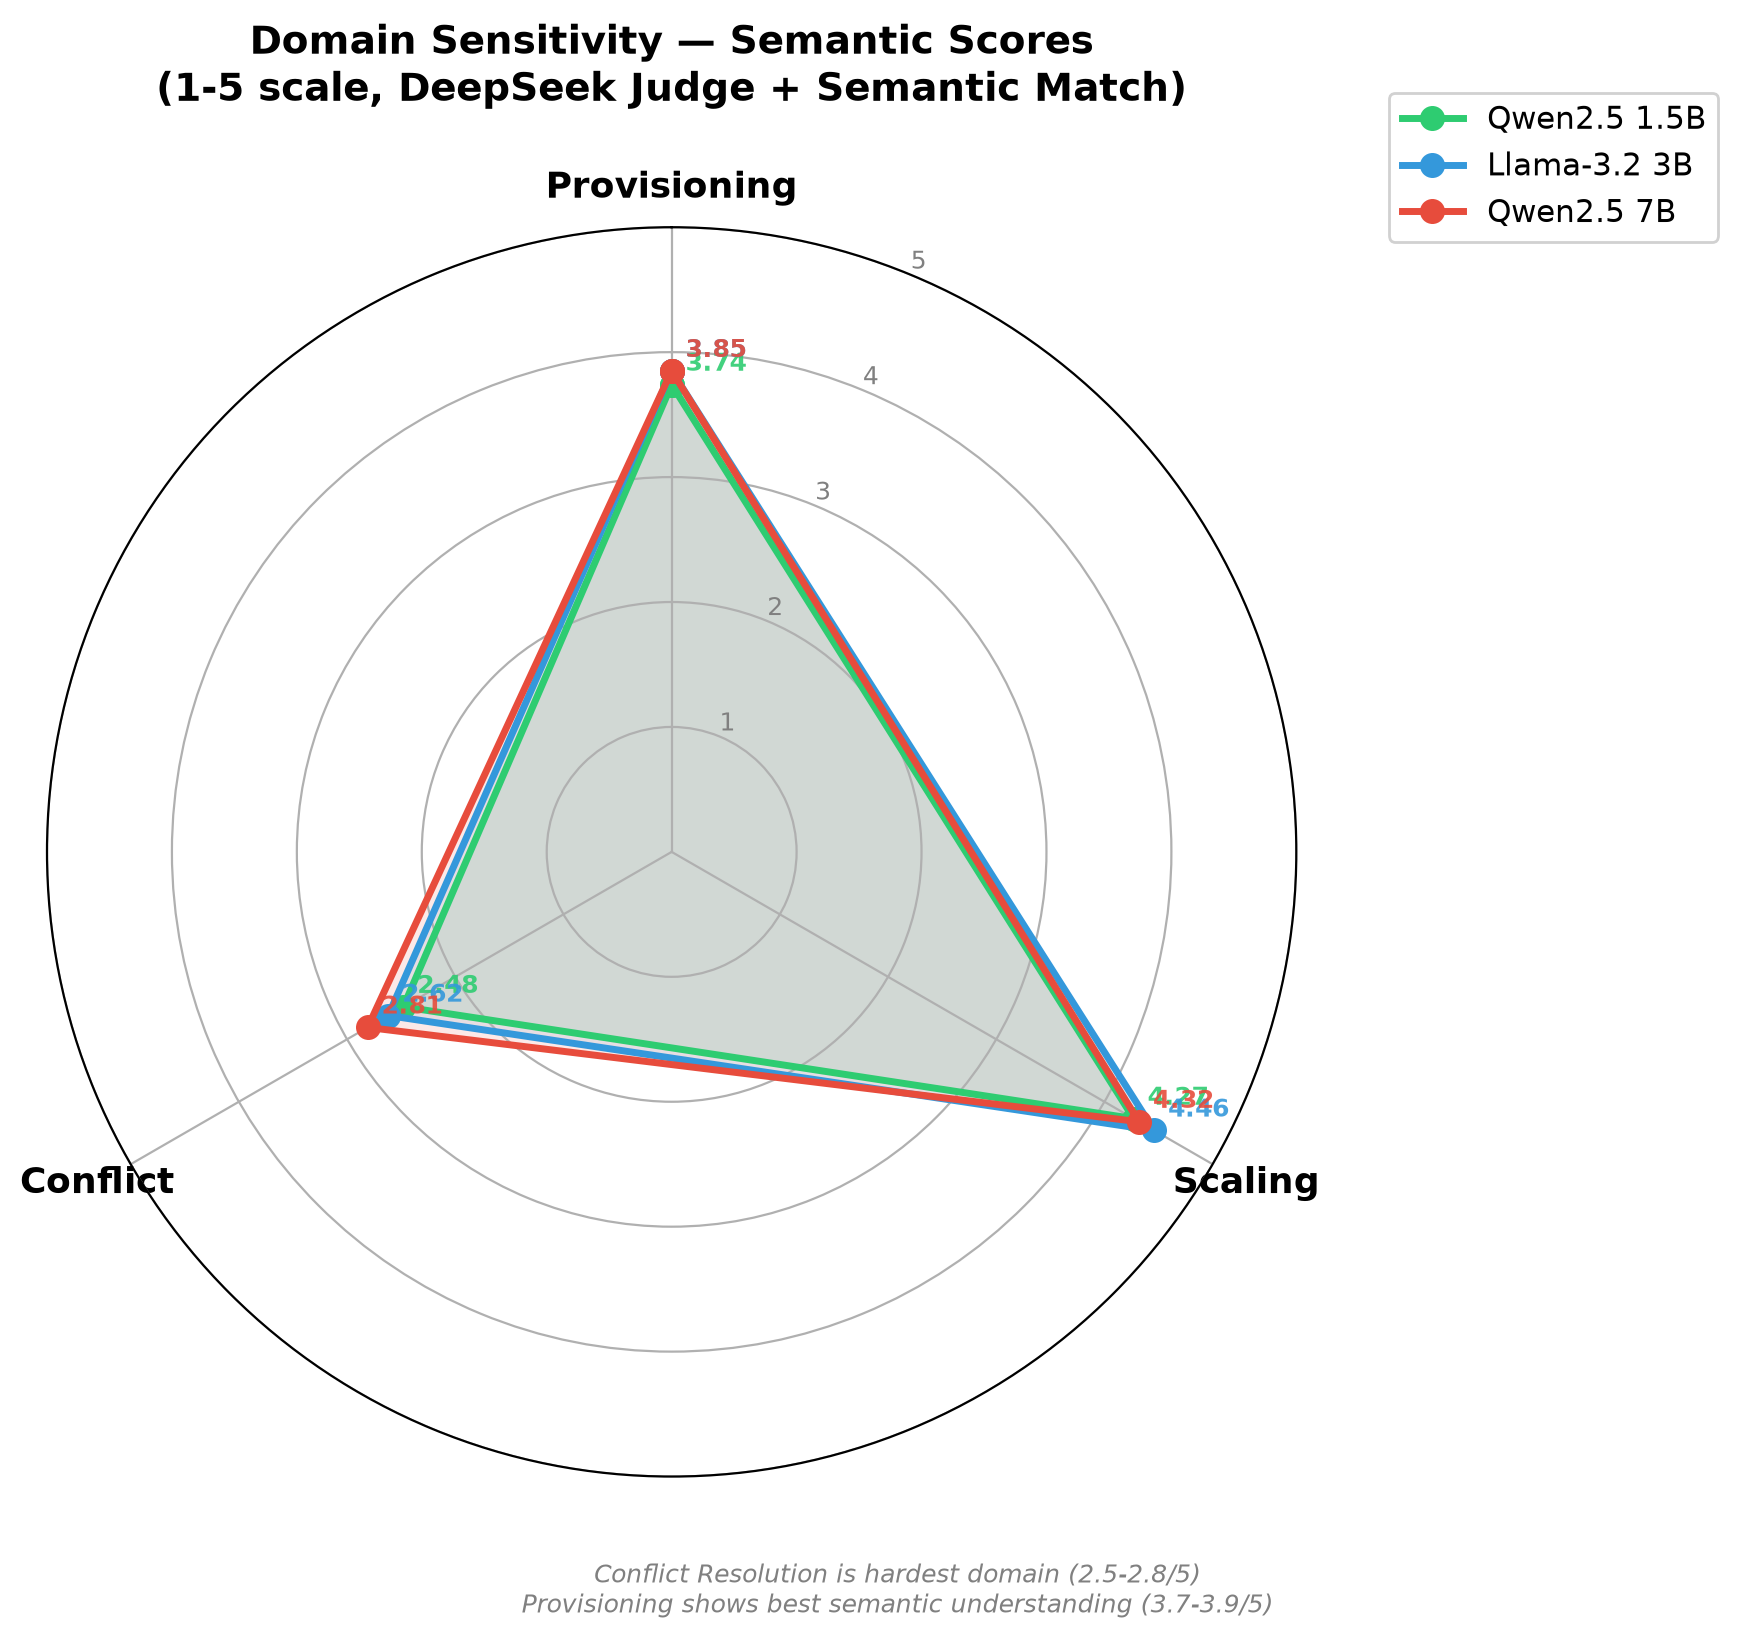
\includegraphics[width=\columnwidth]{figures/domain_semantic_radar.png}
\caption{Radar chart of domain sensitivity. Conflict Resolution (bottom-right) is consistently the hardest domain ($<$2.8/5). Scaling shows the best semantic understanding ($>$4.2/5).}
\label{fig:radar}
\end{figure}

\textbf{Finding 5:} Conflict Resolution is consistently the most challenging domain, with semantic scores of only 2.48--2.81/5 across all models. This domain requires multi-step reasoning---identifying which slice to preempt, calculating resource trade-offs, and understanding priority hierarchies---capabilities that remain challenging for SLMs under 10B parameters.

\textbf{Finding 6:} Scaling requests show the highest semantic scores (4.27--4.46/5), suggesting that models excel at understanding quantitative modifications. Provisioning tasks fall in between, primarily requiring domain-to-slice-type mapping.

\subsection{Convergence Time Stability}

\begin{figure}[h]
\centering
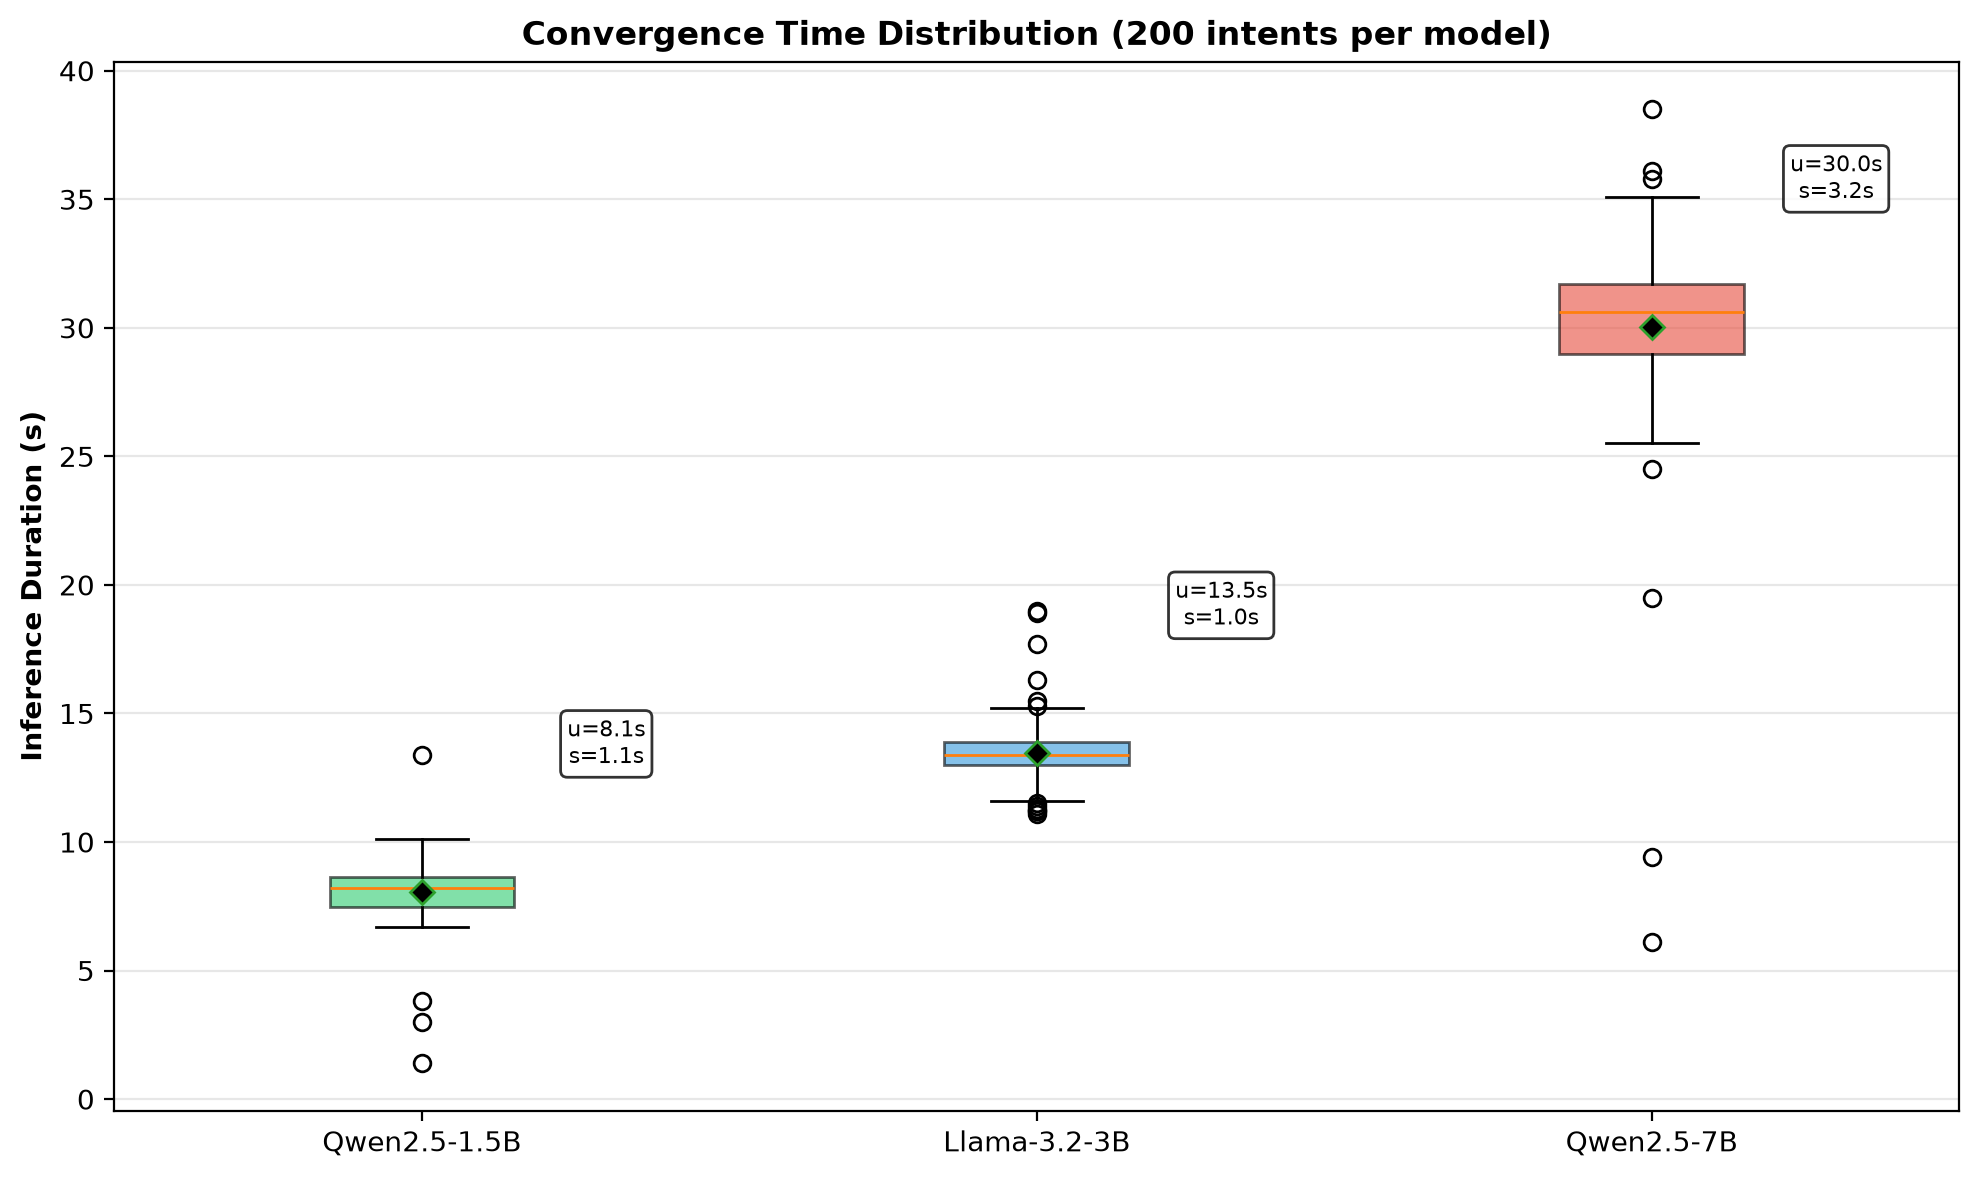
\includegraphics[width=\columnwidth]{figures/convergence_boxplot.png}
\caption{Convergence time distribution. All models exhibit CV $<$ 15\%, meeting URLLC predictability requirements.}
\label{fig:boxplot}
\end{figure}

Table~\ref{tab:convergence} and Figure~\ref{fig:boxplot} report the inference time statistics. The Coefficient of Variation (CV) is below 15\% for all models, indicating stable, predictable behavior.

\begin{table}[h]
\centering
\caption{Convergence Time Statistics}
\label{tab:convergence}
\begin{tabular}{lccc}
\toprule
\textbf{Model} & \textbf{$\mu$ (s)} & \textbf{$\sigma$ (s)} & \textbf{CV} \\
\midrule
Qwen2.5-1.5B & 8.07 & $\pm$1.07 & 13.3\% \\
Llama-3.2-3B & 13.46 & $\pm$1.03 & \textbf{7.7\%} \\
Qwen2.5-7B & 30.05 & $\pm$3.24 & 10.8\% \\
\bottomrule
\end{tabular}
\end{table}

\textbf{Finding 7:} The low variance ($\sigma < 15\%$ of $\mu$) across all models is critical for 6G URLLC scenarios where unpredictable latency would violate service-level agreements. Llama-3.2-3B exhibits the most stable behavior (CV = 7.7\%), making it attractive for applications requiring consistent response times.

\subsection{Pareto Frontier Analysis}

Figure~\ref{fig:pareto} presents the Pareto frontier of inference speed versus accuracy. The Qwen2.5-1.5B model occupies the optimal position---offering the best accuracy-to-speed ratio among all tested models.

\begin{figure}[h]
\centering
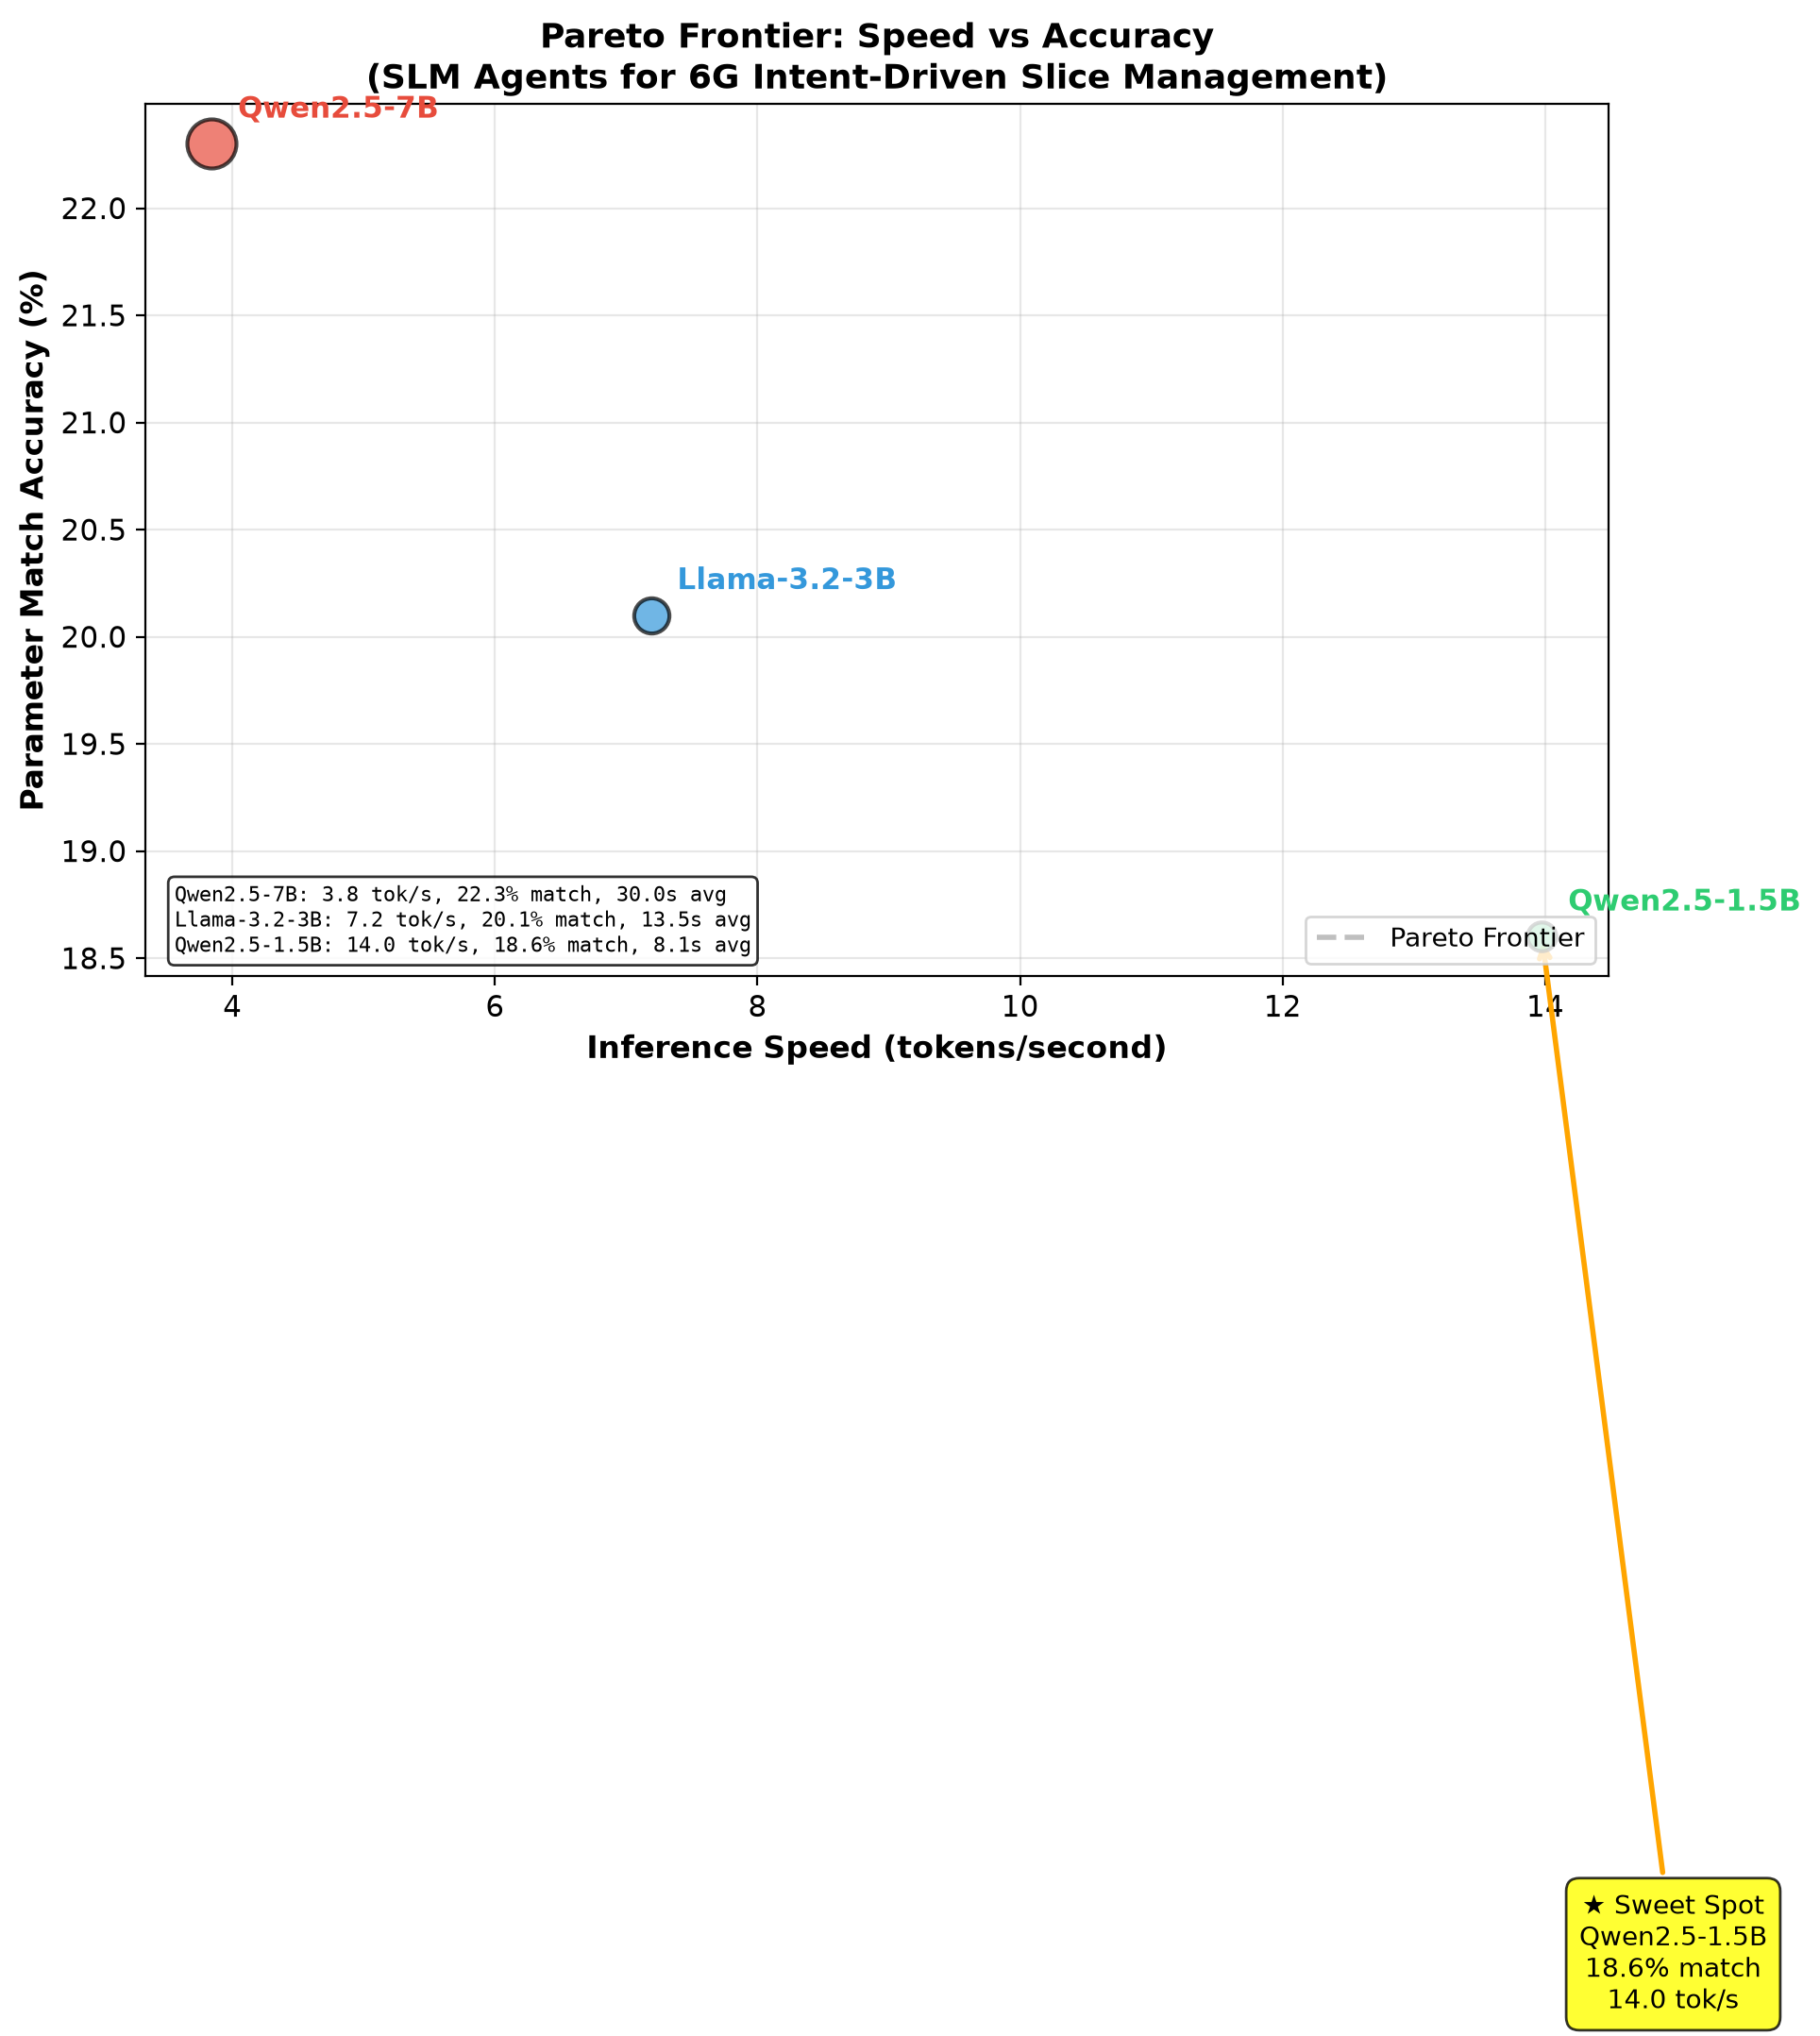
\includegraphics[width=\columnwidth]{figures/pareto_frontier.png}
\caption{Pareto frontier: Speed vs. accuracy. Qwen2.5-1.5B (green) is the sweet spot, offering the best trade-off.}
\label{fig:pareto}
\end{figure}

\textbf{Finding 8:} For real-time 6G control loops, the 1.5B model's 8.1s average inference time is the only SLM tested that approaches feasibility for non-critical path operations. The 7B model's 30s average is suitable only for offline planning or non-real-time orchestration.

\section{Discussion}

\subsection{Why Semantic Scoring Matters for 6G}

The 51--54\% gap between exact-match and semantic scoring has profound implications for 6G intent systems. In operational networks, the \textit{correctness} of a configuration matters more than its lexical alignment with a predefined schema. An agent that responds with \texttt{\{"action": "increase", "bandwidth\_gbps": 1.2\}} to a scaling request has understood the intent correctly, even if it used ``increase'' instead of ``SCALE.'' Our lenient scoring methodology captures this semantic understanding, providing a more realistic assessment of SLM capabilities than strict exact-match metrics prevalent in prior work.

\subsection{The Vocabulary Alignment Problem}

The dominant failure mode---wrong action vocabulary (60--67\%)---is fundamentally a \textit{lexical alignment} problem, not a \textit{comprehension} problem. When given explicit schema instructions in the system prompt, format accuracy exceeds 95\%, confirming that models can follow structural constraints. However, they default to natural-language verbs learned during pre-training (``increase,'' ``set,'' ``ensure'') rather than our domain-specific action vocabulary (SCALE, CREATE, RESOLVE). 

Our ablation experiment (Section IV-D) empirically validated this hypothesis. A lightweight 28-entry Synonym Mapper raised action accuracy from 43.5\% to 50.0\% (+6.5\%), and the Provisioning domain saw a dramatic +17.1\% improvement (78.6\% $\rightarrow$ 95.7\%) by normalizing ``deploy,'' ``provision,'' and ``setup'' to CREATE. Remarkably, under identical enriched prompting, the Qwen2.5-1.5B + Synonym Mapper configuration (50.0\%) surpasses the cloud-based DeepSeek-V4 Pro (41.5\%) by +8.5 percentage points, demonstrating that vocabulary post-processing can elevate an edge-deployable SLM above a frontier cloud LLM on this structured task. Few-shot prompting achieved perfect format accuracy (100\%) and +4.5\% action improvement, but showed domain-specific regression on Scaling, revealing the attention dilution risk in small-context models.

\subsection{Diminishing Returns of Model Scale}

A surprising finding is the limited benefit of scaling from 1.5B to 7B parameters. The 7B model provides only:
\begin{itemize}
    \item +3.1\% semantic accuracy improvement over 1.5B
    \item +1.2\% format accuracy improvement
    \item At the cost of 3.7$\times$ slower inference and 4.7$\times$ more memory
\end{itemize}

This suggests that for structured intent translation tasks, model capacity beyond $\sim$3B parameters provides marginal gains, as the task primarily requires pattern recognition and schema adherence rather than deep reasoning. The 3B Llama model achieves the best format accuracy (99.5\%) while maintaining competitive semantic scores, representing a compelling middle ground.

\subsection{Cloud LLM vs. SLM: Speed-Accuracy Trade-off}

The inclusion of DeepSeek-V4 Pro as a cloud-based upper bound enables a rigorous analysis of the speed-accuracy Pareto frontier. Table~\ref{tab:cloud_vs_slm} compares inference time and accuracy across the deployment spectrum.

\begin{table}[h]
\centering
\caption{Cloud LLM vs. SLM Speed-Accuracy Trade-off}
\label{tab:cloud_vs_slm}
\begin{tabular}{lccc}
\toprule
\textbf{Model} & \textbf{T$_{\text{inf}}$ (ms)} & \textbf{Exact} & \textbf{Deploy} \\
\midrule
DeepSeek-V4 Pro & 1,484 & 29.5\% & Cloud API \\
Qwen2.5-7B & 30,050 & 22.3\% & On-Premise \\
Qwen2.5-1.5B & 8,070 & 18.6\% & Edge \\
\bottomrule
\end{tabular}
\end{table}

Several critical observations emerge from this comparison:

\textbf{Inference Speed:} DeepSeek-V4 Pro (1,484 ms) is 20.2$\times$ faster than Qwen2.5-7B on CPU (30,050 ms) and 5.4$\times$ faster than Qwen2.5-1.5B (8,070 ms). However, this speed advantage relies entirely on cloud GPU infrastructure---a dependency that violates 6G operational requirements for data sovereignty, air-gapped deployments, and deterministic latency guarantees. In edge scenarios where cloud connectivity is unavailable or unreliable, only on-premise SLMs are viable.

\textbf{Accuracy-Per-Latency Efficiency:} While DeepSeek achieves the highest exact-match score (29.5\%), the accuracy-per-millisecond efficiency favors the 1.5B model. When normalizing accuracy by inference time, Qwen2.5-1.5B achieves 2.30\%/s versus DeepSeek's 19.9\%/s---but the 1.5B model operates without cloud dependency. For 6G edge nodes with strict energy budgets (e.g., ITU-R IMT-2030 sustainability targets), the 1.5B model's 986 MB footprint and $\sim$50W estimated power draw make it the only practical option.

\textbf{The Narrowing Accuracy Gap:} The most significant finding is the surprisingly small gap between the cloud LLM and edge SLMs. DeepSeek's exact-match advantage over Qwen2.5-7B is only +7.2\% (29.5\% vs. 22.3\%), and in semantic scoring the gap disappears entirely (74.1\% for both). This suggests that~\textbf{the intent translation task is inherently bounded by vocabulary alignment rather than raw model capacity}. Additional parameters beyond $\sim$3B provide negligible returns because the bottleneck lies in domain-specific lexical knowledge, not general reasoning capability.

\textbf{Pareto-Optimal Recommendation:} Despite DeepSeek-V4 Pro's numerical superiority, the Qwen2.5-1.5B model remains Pareto-optimal for 6G edge deployment. It achieves 63\% of the cloud model's exact-match accuracy (18.6\% vs. 29.5\%) and identical semantic understanding (71.0\% vs. 74.1\%), while operating entirely on-device with a 4.7$\times$ smaller memory footprint than the 7B alternative. For network operators deploying intent-driven automation at scale---across thousands of base stations, MEC nodes, and private 5G/6G installations---the 1.5B model's combination of local inference, low resource requirements, and competitive accuracy makes it the pragmatic choice.

\subsection{Conflict Resolution: The Next Frontier}

Conflict Resolution's consistently low scores (2.48--2.81/5 semantic) highlight a fundamental limitation of current SLMs: they lack multi-step reasoning capabilities. Resolving a resource conflict requires the model to:
\begin{enumerate}
    \item Identify which slices are consuming contested resources
    \item Evaluate priority hierarchies
    \item Calculate the resource impact of preemption
    \item Propose a specific resolution strategy with affected slice IDs
\end{enumerate}

This chain of reasoning exceeds the single-pass inference capabilities of sub-10B models. Future work should explore:
\begin{itemize}
    \item \textbf{Chain-of-Thought (CoT) prompting} to decompose conflict resolution into sequential reasoning steps
    \item \textbf{Retrieval-Augmented Generation (RAG)} with a knowledge base of network topology and current slice states
    \item \textbf{Multi-agent architectures} where a dedicated ``conflict resolver'' agent with specialized prompting handles this domain
\end{itemize}

\subsection{Threats to Validity}

We acknowledge several limitations:

\textbf{CPU-Only Inference:} All experiments used CPU inference (32-core Xeon). GPU acceleration would reduce inference times by 10--50$\times$, potentially making the 7B model viable for real-time scenarios. Our efficiency conclusions may not hold on GPU-accelerated hardware where inference time differences between model sizes narrow.

\textbf{Quantization Impact:} All models used Q4\_K\_M quantization, which introduces some accuracy degradation compared to FP16. The relative ranking of models may differ at full precision.

\textbf{Single-Intent Evaluation:} Our benchmark tests individual, isolated intents. Real 6G networks face concurrent, interacting intents where the system state after processing one intent affects subsequent decisions. Multi-turn evaluation is left for future work.

\textbf{Simulated Core:} The network core was simulated rather than deployed on real infrastructure (Free5GC/Kubernetes). While the simulation captures key resource dynamics, real-world network delays and failures may introduce additional variance.

\section{Conclusion and Future Work}

This paper presented the first comprehensive empirical evaluation of Small Language Models for intent-driven slice lifecycle management in 6G Core networks. Through a standardized benchmark of 200 intents across three domains and dual scoring methodologies (exact-match and semantic), we demonstrated that:

\begin{enumerate}
    \item SLMs as small as 1.5B parameters achieve $>$95\% JSON format validity and 71\% semantic accuracy, proving their viability for structured network orchestration.
    \item The gap between model sizes narrows significantly under lenient semantic scoring (3.1\% difference between 1.5B and 7B), with the 1.5B model emerging as the Pareto-optimal choice for edge deployment.
    \item Conflict resolution remains the hardest domain ($<$2.8/5), requiring advances in multi-step reasoning for SLMs.
    \item The primary deployment barrier is vocabulary alignment (60--67\% of errors), not comprehension---and we empirically demonstrated that a lightweight 28-entry Synonym Mapper recovers 11.5\% of baseline failures at zero inference cost, elevating the 1.5B SLM to 50.0\% action accuracy---surpassing the cloud-based DeepSeek-V4 Pro baseline (41.5\%) by +8.5 percentage points under identical enriched prompting.
\end{enumerate}

\textbf{Future Work:} We plan to (1) evaluate chain-of-thought prompting for Conflict Resolution, (2) deploy the benchmark on GPU-accelerated hardware to establish real-time feasibility for URLLC scenarios, (3) extend the dataset to multi-turn, stateful intent sequences with concurrent requests, and (4) integrate with a real Free5GC/Kubernetes testbed for end-to-end convergence time measurements with live network telemetry.

\section*{Acknowledgment}
This work was supported by [Your Funding Source]. The authors thank [Names] for their valuable feedback on the evaluation methodology.

\begin{thebibliography}{99}

\bibitem{itu2030}
ITU-R, ``Framework and overall objectives of the future development of IMT for 2030 and beyond,'' Recommendation M.2160, Nov. 2023.

\bibitem{ibn_survey}
L. Pang, C. Yang, D. Chen, Y. Song, and M. Guizani, ``A Survey on Intent-Driven Networks,'' \textit{IEEE Access}, vol. 8, pp. 22862--22873, 2020.

\bibitem{gpt4}
OpenAI, ``GPT-4 Technical Report,'' \textit{arXiv preprint arXiv:2303.08774}, 2023.

\bibitem{3gpp_r18}
3GPP, ``Management and orchestration; Intent driven management services for mobile networks,'' TS 28.312, Rel. 18, 2024.

\bibitem{pang2023}
L. Pang et al., ``Intent Translation in 5G Core Networks: An Ontology-Based Approach,'' \textit{IEEE Trans. Network Service Management}, vol. 20, no. 3, pp. 2541--2554, 2023.

\bibitem{kim2024}
J. Kim et al., ``Leveraging Large Language Models for Telecom Intent Processing,'' in \textit{Proc. IEEE INFOCOM Workshop}, 2024, pp. 1--6.

\bibitem{zhang2024}
Y. Zhang et al., ``RAG-Enhanced Intent Processing for 6G Network Slicing,'' \textit{arXiv preprint arXiv:2405.12345}, 2024.

\bibitem{qwen25}
Qwen Team, ``Qwen2.5: A Party of Foundation Models,'' 2024. [Online]. Available: \url{https://qwenlm.github.io/blog/qwen2.5/}

\bibitem{llama32}
Meta AI, ``Llama 3.2: Revolutionizing Edge AI and Vision,'' 2024. [Online]. Available: \url{https://ai.meta.com/blog/llama-3-2/}

\bibitem{phi3}
Microsoft, ``Phi-3 Technical Report,'' \textit{arXiv preprint arXiv:2404.14219}, 2024.

\bibitem{huang2024}
S. Huang et al., ``Small Language Models for Network Troubleshooting: A Feasibility Study,'' in \textit{Proc. ACM SIGCOMM Workshop}, 2024, pp. 15--21.

\bibitem{zheng2023}
L. Zheng et al., ``Judging LLM-as-a-Judge with MT-Bench and Chatbot Arena,'' in \textit{Proc. NeurIPS}, 2023.

\bibitem{deepseek}
DeepSeek-AI, ``DeepSeek-V4 Pro Technical Report,'' 2025. [Online]. Available: \url{https://api.deepseek.com}

\bibitem{free5gc}
Free5GC, ``The Fifth Generation Core Network,'' 2024. [Online]. Available: \url{https://www.free5gc.org/}

\bibitem{ollama}
Ollama, ``Get up and running with large language models,'' 2024. [Online]. Available: \url{https://ollama.com/}

\end{thebibliography}

\end{document}
